\documentclass[tikz,border=10pt]{standalone}
\usepackage{tikz}

\begin{document}
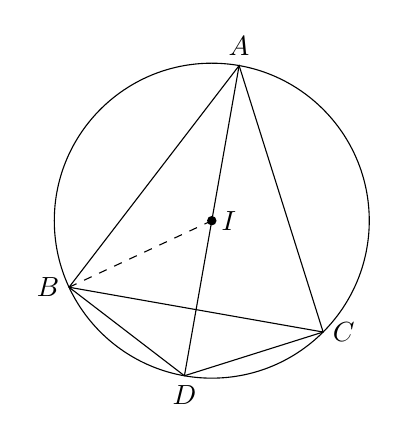
\begin{tikzpicture}[scale=2]
  % Draw the circle
  \draw (0,0) circle (1cm);
  
  % Define points on the circle
  \coordinate (A) at (80:1cm);
  \coordinate (B) at (-155:1cm);
  \coordinate (C) at (-45:1cm);
  \coordinate (D) at (-100:1cm);
  
  % Define center point
  \coordinate (I) at (0,0);
  
  % Draw the inscribed quadrilateral
  \draw (A) -- (B) -- (D) -- (C) -- cycle;
  
  % Draw diagonals
  \draw (A) -- (D);
  \draw (B) -- (C);
  \draw[dashed] (B) -- (I);
  
  % Label the points
  \node[above] at (A) {$A$};
  \node[left] at (B) {$B$};
  \node[right] at (C) {$C$};
  \node[below] at (D) {$D$};
  \node[right] at (I) {$I$};
  \fill (I) circle (0.03);
  
\end{tikzpicture}
\end{document}